%!TEX encoding = UTF-8 Unicode
%!TEX root = ../solutions.tex

\ExerciseSolution{\ExeWeekSIX}

\BasicTasks %%%%%%%%%%%

\Task % uppgift 1

\Subtask Rad 3 och 7 ger båda felmeddelandet "java.lang.NullPointerException". Detta eftersom \code{g} i båda fallen inte innehåller en referens till en \code{Gurka} utan pekar på inget -- "null".

\Subtask 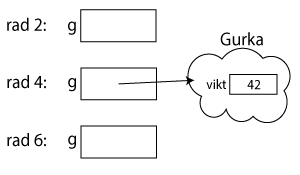
\includegraphics[scale=0.6]{../img/w06-solutions/1b}

\Task % uppgift 2

\Subtask Vi skapar två rymdvarelser, \code{alien} och \code{predator}, med två ben, två armar samt två huvuden (där det ena är skalligt och det andra har hår) vardera. Efter det är varken \code{alien} eller \code{predator} skallig eftersom båda har ett huvud med hår. Sen låter man referensen till \code{predator}s huvud med hår referera till aliens huvud utan hår. Nu är predator helt skallig.

\Subtask  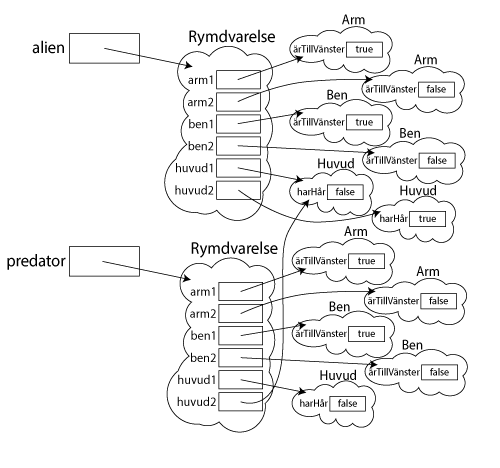
\includegraphics[scale=0.7]{../img/w06-solutions/2b}

\Subtask Eftersom det inte längre finns någon referens som pekar på det objektet kommer Garbage Collector ta hand om det och kommer förr eller senare skrivas över av något annat som behöver sparas. Nej, det går inte att komma åt.

% uppgift 3
\Task Rad 2: 
\begin{REPL}
	error: value vikt is not a member of Gurka1
\end{REPL}
Detta eftersom om man varken väljer att skriva \code{val} eller \code{var} skapar inte scala någon getter eller setter (metoder för att läsa/ändra en variabel) och därför ser det ut som att vikt inte finns för kompilatorn.

Rad 4: Denna rad skapar inte en error eftersom om man skriver \code{val} innan variabeln skapas en getter automatiskt och man kan därför komma åt \code{vikt}.

Rad 6: 
\begin{REPL}
	error: value vikt in class Gurka3 cannot be accessed in Gurka3
\end{REPL} 
I detta fallet skapas en \code{getter} men eftersom accessnivån sätts till \code{private} vet kompilatorn att man inte får komma åt variabeln utifrån.

Rad 11: 
\begin{REPL}
	java.lang.NullPointerException
\end{REPL} 
Detta eftersom \code{kompis} är \code{ingenGurka} som inte pekar på något objekt och när man då försöker komma åt ett attribut från den kommer det inte funka.

Rad 12: Kommer inte generera en error eftersom när man kallar \code{kompisVikt} (som är \code{public}) försöker den komma åt \code{Gurka4(84, null).vikt}. \code{vikt} är \code{private val} vilket innebär att det har en getter och eftersom huvudobjektet också är av typen \code{Gurka4} är accessnivån tillräckligt hög.

Rad 13: 
\begin{REPL}
	error: value vikt is not a member of Gurka5
\end{REPL} 
När man sätter ett attribut till \code{private[this]} tillåts inte ens objekt av samma typ att komma åt variabeln och därför får man en error som säger att den inte finns.

Rad 17: 
\begin{REPL}
	error: constructor Gurka6 in class Gurka6 cannot be accessed in object
\end{REPL} 
Eftersom man satt klassparametrarna till \code{private} kan man inte komma åt konstruktorn och därför får man en error.

Rad 26: 
\begin{REPL}
	error: constructor Gurka7 in class Gurka7 cannot be accessed in object
\end{REPL} 
Samma anledning som på rad 17.

Rad 27: 
\begin{REPL}
	java.lang.IllegalArgumentException: requirement failed: negativ vikt: -42
\end{REPL} 
Kompanjonsobjektet har en requirement på att \code{vikt >= 0} vilket innebär att om det inte stämmer kommer man få en error av typen \code{IllegalArgumentException}.

Rad 30: Anledningen till att man kan sätta vikten till något negativt är att checken om det är negativt endast görs när man skapar \code{Gurka7} vilket innebär att i efterhand kan man ändra den till vilket värde som helst (av typen \code{Int}).

\Task % uppgift 4

\Subtask Rad 16: 
\begin{REPL}
	java.lang.IllegalArgumentException: requirement failed: negativ vikt: -42
\end{REPL} 
Kompanjonsobjektet har en requirement på att \code{vikt >= 0} vilket innebär att om det inte stämmer kommer man få en error.

Rad 20: 
\begin{REPL}
	java.lang.IllegalArgumentException: requirement failed: negativ vikt: -1
\end{REPL} 
Eftersom settern har implementerat ett krav på att vikten måste vara större eller lika med 0 får man en error när man försöker sätta den till -1.

Rad 22: 
\begin{REPL}
	java.lang.IllegalArgumentException: requirement failed: negativ vikt: -958
\end{REPL} 
Eftersom 42-1000 är mindre än noll får man en error.

\Subtask Man kan sätta egna mer specifika krav på vad som får göras med värdena så man har större koll på att inget oväntat händer.

% uppgift 5
\Task \begin{CodeSmall}
	class Square(val x: Int, val y: Int, val side: Int) {
		val area: Int = side*side
		
		def move(dx: Int, dy: Int): Square = new Square(x + dx, y + dy, side)
		
		def isEqualSizeAs(that: Square): Boolean = this.side == that.side
		
		def scale(factor: Double): Square = new Square(x, y, (side*factor).toInt)
		
		override def toString: String = s"Square(x: $x, y: $y, side: $side)"
	}
	
	object Square {
		val unit: Square = new Square(0, 0, 1)
		
		def apply(x: Int, y: Int, side: Int): Square = new Square(x, y, side)
		
		def apply(): Square = new Square(0, 0, 1)
	}
\end{CodeSmall}

Eftersom \code{s1}, \code{s2}, \code{s3} och \code{Square.unit} alla har en sida med längden 1 så kommer rad 3-5 returnera \code{true}. Rad 6 kommer returnera \code{false} eftersom \code{s2.scale(math.Pi)} sida är $\pi$ och \code{s2} fortfarande har sidan 1. Rad 7 kommer däremot returnera \code{true} då båda har sidan $\pi$.

\Task % uppgift 6

\Subtask Variablerna \code{a} och \code{b} är båda objekt av en vanlig klass vilket kommer innebära att de jämförs med referenslikhet och eftersom de inte är samma objekt retunerar \code{==} \code{false}. \code{c} och \code{d} är däremot objekt av en case klass så de jämförs med strukturlikhet och eftersom de har samma vikt returnerar \code{==} \code{true}.

\Subtask Både \code{a eq b} och \code{c eq d} ska returnera \code{false} eftersom de alla är olika objekt och det är referenslikhetsom gäller.

\Task % uppgift 7

\Subtask se e) för komplett lösning

\Subtask se e) för komplett lösning

\Subtask se e) för komplett lösning

\Subtask se e) för komplett lösning

\Subtask \begin{CodeSmall}
case class Point(x: Int, y: Int) {
	
	def distanceTo(that: Point): Double = math.hypot(that.x - x, that.y -y)
	
	def distanceTo(x: Int, y: Int): Double = distanceTo(Point(x, y))
	
	def move(dx: Int, dy: Int): Point = Point(x + dx, y + dy)
}

object Point {
	//val origin: Point = new Point(0, 0)
	def origin: Point = Point(0, 0)
}
\end{CodeSmall}

\Subtask \code{==} och \code{!=} kollar strukturlikhet så om två objekt innehåller samma värden kommer \code{==} returnera \code{true} och \code{!=} \code{false} och vise versa. \code{eq} och \code{ne} kollar referenslikhet så om två variabler pekar på samma objekt kommer \code{eq} returnera \code{true} och \code{ne} \code{false} och vise versa.

\Subtask \code{false}. Detta eftersom om origin implementeras som en metod som returnerar en ny \code{Point} varje gång den kallas kommer \code{Point.origin} inte peka på samma objekt varje gång metoden kallas (\code{eq} är referenslikhet).

\Subtask Sturkturlikhet bryr sig endast om innehållet i objekten och jämför det. Det kvittar alltså om det är samma objekt eller två olika så länge de innehåller samma värden. Referenslikhet kollar endast på om det är samma objekt variablerna pekar på och struntar fullständigt i om de innehåller samma värden.

% uppgift 8
\Task \begin{CodeSmall}
class Square(val p: Point, val side: Int) {
	val area: Int = side*side
	
	def move(dx: Int, dy: Int): Square = new Square(p.move(dx, dy), side)
	
	def isEqualSizeAs(that: Square): Boolean = this.side == that.side
	
	def scale(factor: Double): Square = new Square(p, (side*factor).toInt)
	
	override def toString: String = s"Square(p: $p, side: $side)"
}

object Square {
	val unit: Square = new Square(new Point(0, 0), 1)
	
	def apply(x: Int, y: Int, side: Int): Square = 
		new Square(new Point(x, y), side)
	
	def apply(): Square = new Square(new Point(0, 0), 1)
}
\end{CodeSmall}

% uppgift 9
\Task  \begin{CodeSmall}
case class Point(p:(Int,Int)) {
	val x: Int = p._1
	
	val y: Int = p._2
	
	def distanceTo(that: Point): Double = math.hypot(that.x - x, that.y -y)
		
	def distanceTo(that: (Int, Int)): Double = distanceTo(Point(that))
	def move(dx: Int, dy: Int): Point = Point(x + dx, y + dy)
}

object Point {
	val origin: Point = new Point(0, 0)
}
\end{CodeSmall}

% uppgift 10
\Task Inget! Eftersom både \code{Point(1,2)} och \code{Point((1,2))} är okej sätt att komma åt den nya klassen så kommer det se likadant utifrån och därför behöver man inte ändra något i \code{Square}. 

\Task % uppgift 11

\Subtask \begin{CodeSmall}
class Frog private (initX: Int = 0, initY: Int = 0) {
	private var _x: Int = initX
	private var _y: Int = initY
	private var _distanceJumped: Double = 0
	
	def jump(dx: Int, dy: Int): Unit = {
		_x += dx
		_y += dy
		_distanceJumped += Math.hypot(dx, dy)
	}
	
	def x: Int = _x
	def y: Int = _y
	
	def randomJump: Unit = {
		val r = scala.util.Random
		val xtmp = r.nextInt(10)+1
		val ytmp = r.nextInt(10)+1
		_x += xtmp
		_y += ytmp
		_distanceJumped += Math.hypot(xtmp, ytmp)
	}
	
	def distanceToStart: Double = Math.hypot(_x,_y)
	def distanceJumped: Double = _distanceJumped
	def distanceTo(that: Frog): Double = Math.hypot(_x - that.x, _y - that.y)
}

object Frog {
	def spawn(): Frog = new Frog()
}
\end{CodeSmall}

\Subtask \begin{CodeSmall}
val f1 = Frog.spawn()
//test requirement 1 and 4
assert(f1.x == 0 && f1.y == 0, "Either x or y isn't 0")

f1.jump(4,3)
//test requirement 1 and 5
assert(f1.x == 4 && f1.y == 3, "Either x isn't 4 or y isn't 3")

f1.jump(4,3)
//test requirement 2
var text = "distanceJumped is " + f1.distanceJumped + ". Should be 10"
assert(f1.distanceJumped == 10, text)

f1.jump(-4,-3)
//test requirement 3
text = "distanceToStart is " + f1.distanceJumped + ". Should be 5"
assert(f1.distanceToStart == 5, text)

var f2 = Frog.spawn()
for (x <- 1 to 1000) {
	f2.randomJump
	//test requirement 5
	text = "Either x or y isn't in [1,10]. x:" + f2.x + ", y: " + f2.y
	assert(f2.x > 0 && f2.x <= 10 && f2.y > 0 && f2.y <= 10, text) 
	f2 = Frog.spawn()
}

val f3 = Frog.spawn()
f3.jump(1,1)
val f4 = Frog.spawn()
f4.jump(4,5)
// Test distanceT()
text = "distanceTo is " + f3.distanceTo(f4) + ". Should be 5"
assert(f3.distanceTo(f4) == 5, text)
\end{CodeSmall}

\Subtask Getter

\Subtask Om metoden har parametrar och retur-typen \code{Unit}. Det betyder troligen att parametrarna ändrar något istället för att skapa något nytt.

\Subtask \begin{CodeSmall}
class Frog private (initX: Int = 0, initY: Int = 0) {
	private var _x: Int = initX
	private var _y: Int = initY
	private var _distanceJumped: Double = 0
	
	def jump(dx: Int, dy: Int): Unit = {
		_x += dx
		_y += dy
		_distanceJumped += Math.hypot(dx, dy)
	}
	
	def x: Int = _x
	def y: Int = _y
	
	def x(newX: Int): Unit = {
		_distanceJumped += Math.abs(_x - newX)
		_x = newX
	} 
	def y(newY: Int): Unit = {
		_distanceJumped += Math.abs(_y - newY)
		_y = newY
	} 
	
	def randomJump: Unit = {
		val r = scala.util.Random
		val xtmp = r.nextInt(10)+1
		val ytmp = r.nextInt(10)+1
		_x += xtmp
		_y += ytmp
		_distanceJumped += Math.hypot(xtmp, ytmp)
	}
	
	def distanceToStart: Double = Math.hypot(_x,_y)
	def distanceJumped: Double = _distanceJumped
	def distanceTo(that: Frog): Double = Math.hypot(_x - that.x, _y - that.y)
}

object Frog {
	def spawn(): Frog = new Frog()
}
\end{CodeSmall}

\Subtask \begin{CodeSmall}
var noCollision = true
var counter = 0
val numberOfFrogs = 100
val distanceBetweenFrogs = 8
val frogArray = Array.fill(numberOfFrogs){Frog.spawn()}
(0 until numberOfFrogs).foreach(i => frogArray(i).x(i*distanceBetweenFrogs))
while (noCollision) {
	frogArray.foreach(frog => frog.randomJump)
	for (frog <- frogArray) {
		for (frog2 <- frogArray) {
			if (frog != frog2 && frog.distanceTo(frog2) < 0.5) {
				noCollision = false
			}
		}
	}
	counter += 1
} 
print(counter)
\end{CodeSmall}


\clearpage

\ExtraTasks %%%%%%%%%%%%

\Task 

\vspace{1em} %tweak pagination

\begin{CodeSmall}
/** A mutable and expensive Square. */
class Square private (val initX: Int, val initY: Int, val initSide: Int) {
  
  private var nMoves = 0;
  private var sumCost = 0.0;
  private var _x = initX;
  private var _y = initY;
  private var _side = initSide;
  
  private def addCost: Unit = { 
   sumCost += math.hypot(x - initX, y - initY) * side
  }
  
  /** The current position on the x axis */
  def x: Int = _x

  /** The current position on the y axis */
  def y: Int = _y

  /** The size of the side */
  def side = _side

  /** Scales the size of this square and rounds it to nearest integer */
  def scale(factor: Double): Unit = { _side = (_side * factor).round.toInt }

  /** Moves this square to position (x + xd, y + dy) */
  def move(dx: Int, dy: Int): Unit = { 
    _x += dx; _y += dy; 
    nMoves += 1
    addCost
  }

  /** Moves this square to position (x, y) */
  def moveTo(x: Int, y: Int): Unit = { 
    _x = x; _y = y; 
    nMoves += 1
    addCost
  }
  
  /** The accumulated cost of this Square */
  def cost: Double = sumCost

  /** Reset the cost of this Square */
  def pay: Unit = {sumCost = 0}
  
  /** A string representation of this Square */
  override def toString: String = 
    s"Square[($x, $y), side: $side, #moves: $nMoves times, cost: $sumCost]"
}

object Square {
  private var created = Vector[Square]()
 
  /** Constructs a new Square object at (x, y) with size side */
  def apply(x: Int, y: Int, side: Int): Square = {
    require(side >= 0, s"side must be positive: $side")
    val sq = (new Square(x, y, side))
    created :+= sq
    sq
  }

  /** Constructs a new Square object at (0, 0) with side 1 */
  def apply(): Square = apply(0, 0, 1)

  /** The total number of moves that have been made for all squares. */
  def totalNumberOfMoves: Int = created.map(_.nMoves).sum
  
  /** The total cost of all squares. */  
  def totalCost: Double = created.map(_.cost).sum
} 
\end{CodeSmall}

\AdvancedTasks %%%%%%%%%

\TODO